%\chapter{開発プロセス}
\section{第1サイクル(5月1日〜7月3日)}

\begin{description}
\item[第1回フィールドワーク]\mbox{}
\end{description}
 我々は木古内町の観光産業と開発するアプリの方向性を考えるにあたり、木古内町観光の解決すべき問題点の発見を目的として木古内町でフィールドワークを行った。このフィールドワークでは、多角的に木古内町を観察するために函館市-木古内町間の交通手段をメンバー間で電車・自転車・車の3つに分担し、それぞれが観光者の視点に立って行った。木古内町でのフィールドワークを行って気づいたことは主に2点あり、まず1点目は、木古内町の観光情報が分散して存在していることである。そのため、木古内町に着いた際、どこで何ができるのか分かりにくかった。これは、前述の木古内町観光協会WebサイトやSNS、パンフレットなど多くのメディアで情報が発信されていることで観光情報が分散していて観光者に伝わっていないことや、情報提供するコンテンツが木古内の魅力的な部分を十分に伝えていないことが原因だと考えられる。気づいたことの2点目は、観光を終えた人々には観光の体験や思い出を友人などの親しい人に伝えたいというモチベーションがあるという点である。観光の体験や思い出を伝えるという行為には、その相手に観光地の良さ伝え、新たな観光客を呼び込む手がかりとなる要素を含んでおり、それをより魅力的に伝えるには写真を使うのが効果的である。しかしながら、多くの観光者はその写真はあまり整理を行っておらずそれを効果的に伝えられていない。以上の気づきを元に第1サイクルの開発を開始した。
\bunseki{細川椋太}

第1サイクルはプロジェクト発足から中間発表会用のポスターレビューまでとした。本サイクルでは第1回フィールドワークの経験から、木古内町の観光情報が分散していること、観光中に撮影した写真が整理されていないことを問題として定義した。最初の設計段階であがった案は以下の5つであり具体的な画面イメージを作成できたのはマップ画面、Webページを表示する画面、お散歩コースを表示する画面の3つである。これらの案に対するレビューを6月12日に企業講師の方から受けた結果、現在の提案に木古内らしさを加える必要があるとの指摘を受けた。
\begin{description}
\item[初期段階でのアプリ機能案]\mbox{}
\begin{itemize}
 \item マップ上に表示されたピンをタップすると吹き出しを表示し、吹き出し内に観光スポッ ト名やお店の営業時間および連絡先を表示する機能
  \item 吹き出しをタップするとお店のWebページへ画面遷移する機能
 \item 木古内町民しか知らないニュースや、木古内町の天気をマップ画面に表示する機能
 \item ユーザ同士で木古内町の写真を共有できる機能
 \item 木古内町観光協会が公開している木古内お散歩コースをマップの中に盛り込む
\end{itemize}
\end{description}

以下に示す図5.1は作成した画面のイメージである。図5.1(a)は、マップ上にピンが自動的に配置され、そのピンをタップした時に表示する画面のイメージである。この画面では観光スポットを検索できたり木古内町の天気を表示したり、表示するピンのカテゴリを切り替えることができる。図5.1(b)は、図5.1(a)に表示している吹き出しをタップすると画面遷移して表示する画面のイメージである。ここには、観光スポットの詳細情報としてお店のメニューや営業時間、商品の写真などを記載する機能がある。図5.1(c)は、木古内町観光協会が公開しているお散歩コースを表示している画面イメージである。画面下のタブをタップして選択すると表示するコース内容を対応するコース内容へ切り替えることができる。また、画面上にはお散歩コースの途中にある観光スポットを赤点で表示しており、その赤点をタップすると図5.1(a)と同様に吹き出しと対応する情報を表示する機能が備わっている。

\begin{figure}[htbp]
  \begin{center}
    \begin{tabular}{c}

      % 1
      \begin{minipage}{0.33\hsize}
        \begin{center}
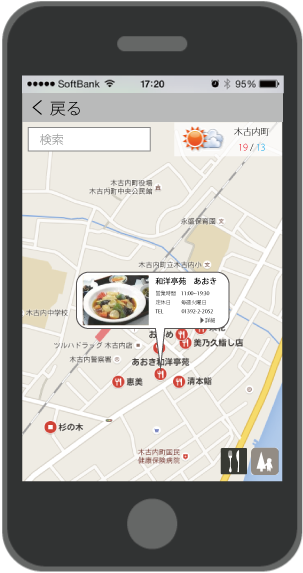
\includegraphics[width=4cm, bb=0 0 303 573]{5.2_map1.png}
          \hspace{1cm} (a)観光スポットの紹介
        \end{center}
      \end{minipage}

      % 2
      \begin{minipage}{0.33\hsize}
        \begin{center}
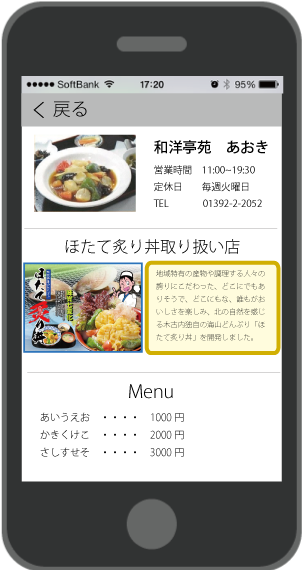
\includegraphics[width=4cm, bb=0 0 304 570]{5.2_map2.png}
          \hspace{1cm} (b)観光スポットの詳細情報
        \end{center}
      \end{minipage}

      % 3
      \begin{minipage}{0.33\hsize}
        \begin{center}
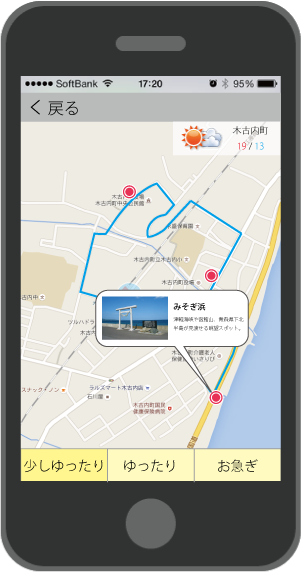
\includegraphics[width=4cm, bb=0 0 302 572]{5.2_sanpo.png}
          \hspace{1cm} (c)お散歩コース
        \end{center}
      \end{minipage}

    \end{tabular}
    \caption{初期段階での画面イメージ}
    \label{fig:lena}
  \end{center}
\end{figure}

その後は上記の初期段階でのアプリ機能案に対して議論を行い、木古内町民しか知らないニュースは継続運用が困難であるという理由から実装を保留した。また、木古内町観光協会が公開している木古内お散歩コースをマップの中に盛り込む機能も実装を保留した。理由は、公開されていたコース内容が車での移動を前提にしており、車を運転しながらスマートフォンを見ることになるため同伴者が必要という縛りを設けてしまうからである。この段階で実装した機能は下記の4つである。1つ目は、マップ上に表示されたピンをタップすると吹き出しを表示し、吹き出し内に観光スポッ ト名やお店の名前および連絡先を表示する機能である(図5.2(a)参照)。2つ目はカテゴリごとにピンの表示を切り替える機能である(図5.2(a)参照)。3つ目は、現在地から目的地までのルート案内を行う機能である(図5.2(b)参照)。4つ目は、木古内町の天気を表示する機能である(図5.2(c)参照)。上記4つの機能に対してチーム内で中間発表会に展示する内容として不足はないと判断したが、中間発表会用のポスターレビューの際にユーザストーリに問題があるとの指摘を受けた。指摘の内容は、観光客は観光スポットやランドマークの写真を見てからその場所へ行くのが通常の流れであるが、当時作成していたアプリは場所を伝えてから写真や詳細情報を見せる流れになっており、情報を提供する順番が逆である。この状態だと木古内町の魅力はもちろんのこと、何があるかすら伝わらないとの内容であった。この指摘を受けて先に伝える情報は場所ではなく内容にすべきであるという結論に達した。そして中間発表会までに改善することをチーム内で合意し、第2サイクルへ移行した。\par

最後に、本サイクルで実装した4つの機能を実行している時の画面を図5.2に示し、それらについて詳細を述べる。1つ目の機能と2つ目の機能を実行している画面は図5.2(a)である。この画面はユーザが一番最初に見る画面である。この画面ではマップ上に表示されたピンタップすることで、観光スポットの名前またはお店の名前と連絡先が記載してある吹き出しを表示することができる。また、画面下に表示している食べる、見る、買うの3つのカテゴリボタンをタップすることで対応するカテゴリのピンをマップ上に表示することができる。図5.2(b)は3つ目の機能を実行している時の画面である。図5.2(a)中にある吹き出し右側に表示している青いアイコン i をタップすることで現在地から対応する場所までのルートが赤線で表示される。なお、図5.2(b)は木古内駅を現在地として設定している状態である。図5.2(c) は、木古内町の天気を表示している画面である。現在の最高気温および最低気温、3 時間ごとの天気、1 週間の天気予報を表示している。

\begin{figure}[htbp]
  \begin{center}
    \begin{tabular}{c}

      % 1
      \begin{minipage}{0.33\hsize}
        \begin{center}
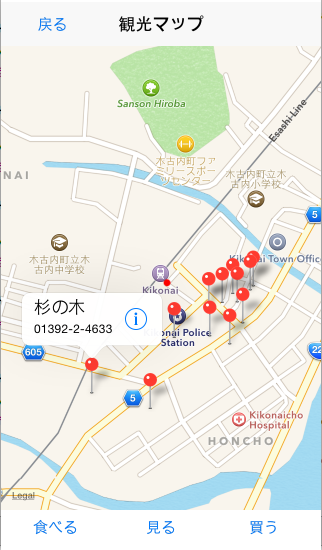
\includegraphics[width=4cm, bb=0 0 322 550]{5.3_map1.png}
          \hspace{1cm} (a)詳細情報のクイック表示
        \end{center}
      \end{minipage}

      % 2
      \begin{minipage}{0.33\hsize}
        \begin{center}
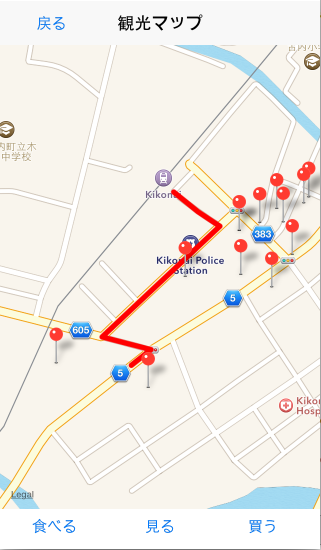
\includegraphics[width=4cm, bb=0 0 321 550]{5.3_map2.png}
          \hspace{1cm} (b)ルート案内
        \end{center}
      \end{minipage}

      % 3
      \begin{minipage}{0.33\hsize}
        \begin{center}
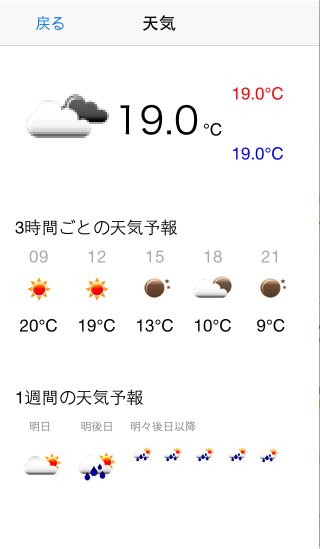
\includegraphics[width=4cm, bb=0 0 320 549]{5.3_weather.png}
          \hspace{1cm} (c)木古内町の天気を表示
        \end{center}
      \end{minipage}

    \end{tabular}
    \caption{第1サイクルでの完成画面 }
    
    \label{fig:lena}
  \end{center}
\end{figure}
\bunseki{岩見建汰}